% ---------------------------------------------------------------------- %

\documentclass[letterpaper,10pt]{article}



\pagestyle{empty}

\usepackage[table]{xcolor}
\usepackage{color, colortbl}
\usepackage{tabularx}
\usepackage{amssymb}
\usepackage{enumerate}

\definecolor{LightGray}{gray}{0.9}

\usepackage{amsmath}
\usepackage{amscd}
\usepackage{url}

\usepackage{graphicx}


\title{Installing AIMBAT}
\author{Northwestern Seismology Group}
\date{\today}

\begin{document}
\maketitle

% ************************************************************* %
%                                                               %
%                       OPERATING SYSTEM                        %
%                                                               %
% ************************************************************* %

\section{Getting your Operating System}

Go to \verb"System Preferences" as in~\ref{fig:system_preferences}, and click on \verb"Startup Disk". It should show your operation system version.

\begin{figure}[h!]
  \centering
  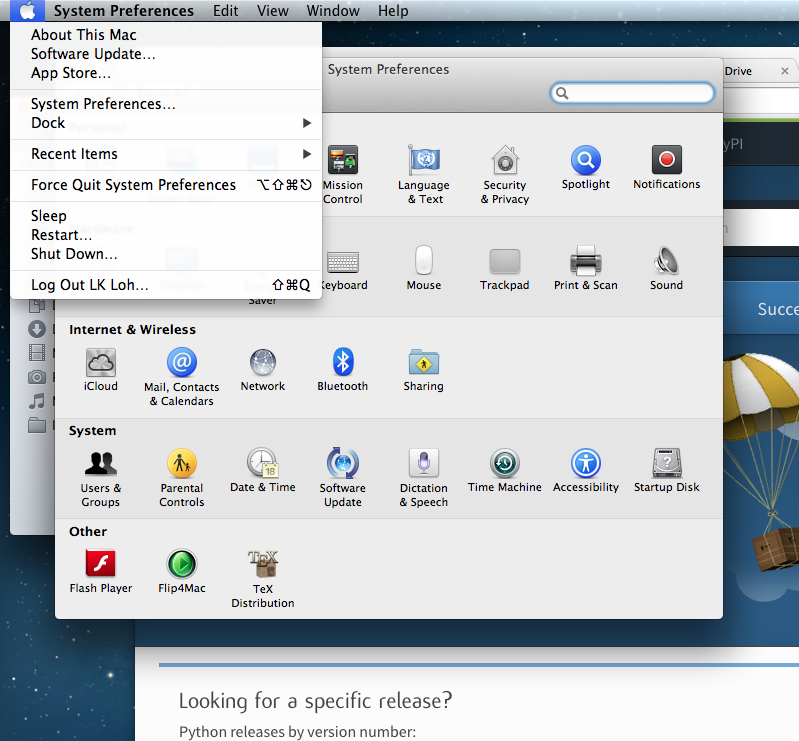
\includegraphics[width=0.5\textwidth]{images/system_preferences}
  \caption{Console}
  \label{fig:system_preferences}
\end{figure}

\begin{figure}[h!]
  \centering
  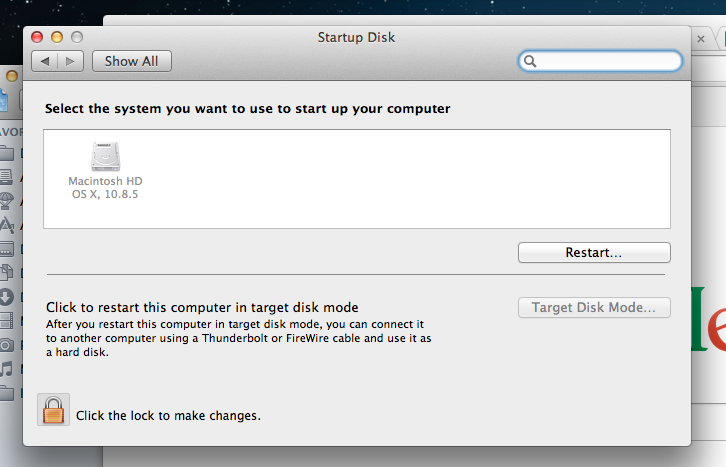
\includegraphics[width=0.5\textwidth]{images/startup_disk}
  \caption{Console}
  \label{fig:startup_disk}
\end{figure}

% ************************************************************* %
%                                                               %
%                       OPERATING SYSTEM                        %
%                                                               %
% ************************************************************* %

% ************************************************************* %
%                                                               %
%                       INSTALLING PYTHON                       %
%                                                               %
% ************************************************************* %

\section{Installing Python}

% ------------------------------------------------------------- %

\subsection{Installing Packages with Enthought Canopy}

Someone suggested Enthought Canopy to install all the Python packages easily. See here for his website. \url{http://www1.i2r.a-star.edu.sg/~lins/codes/python.html}. If you download the free version of Enthought Canopy, it gives you everything you need for installing AIMBAT properly. If you do not want to use Enthought Canopy, read the rest of this section to use Macports or Pip. 

\begin{figure}[h!]
  \centering
  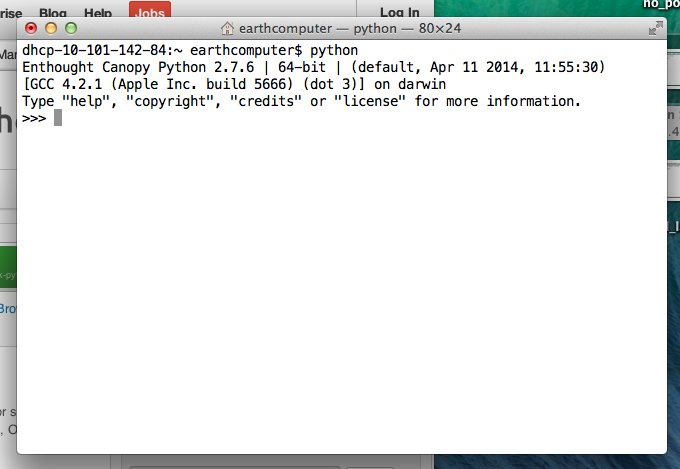
\includegraphics[width=0.5\textwidth]{images/enthought_console}
  \caption{Console}
  \label{fig:enthought_console}
\end{figure}

% ------------------------------------------------------------- %

\subsection{Installing with Pip}

Using Enthought Python is recommended, and it is assumed that readers of this section have a version of python on their computer they already want to keep.

For those who do not want to use Enthought Python, get Python straight from the official website here: \url{https://www.python.org/download}.  Make sure to get version 2.7 and above. If you install a 2.7 and that is a higher version that one you already have, version 2.7 should be used by default when you fire up python. 

Install pip on the Mac. To do so, in terminal type \texttt{python get-pip.py} to download the package manager pip.

Install the rest of the packages.
\begin{verbatim}
  sudo pip install numpy
  sudo pip install ipython
  sudo pip install matplotlib
\end{verbatim}

Scipy is more tricky to install, as it depends on having gfortran. Try downloading the package directly, instead of using a package manager: \url{http://sourceforge.net/projects/scipy/files/scipy/0.9.0/}.

\begin{figure}[h!]
  \centering
  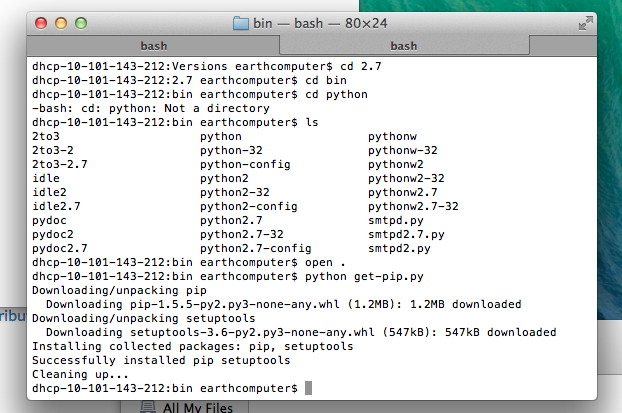
\includegraphics[width=0.5\textwidth]{images/getting_pip}
  \caption{Getting pip}
  \label{fig:getting_pip}
\end{figure}

% ------------------------------------------------------- %

\subsection{Installing with Macport}

Usually, Macs already have python installed by default. To check if you have python on your mac,
open up terminal, and do python in the terminal. If python is installed you should see some souch of console show up, as in Figure~\ref{fig:python_console}. If python is not installed, you should see an error message show up. 

\begin{figure}[h!]
  \centering
  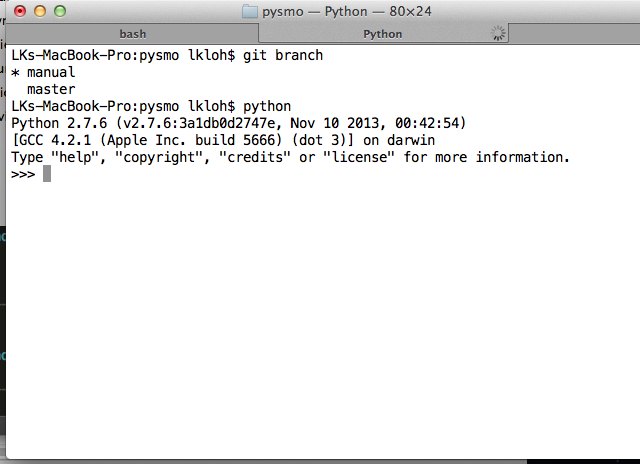
\includegraphics[width=0.5\textwidth]{images/python_console}
  \caption{Console}
  \label{fig:python_console}
\end{figure}

To get python, go to \url{https://www.python.org/}, and get the correct version for your operatin system. 

\begin{figure}[h!]
  \centering
  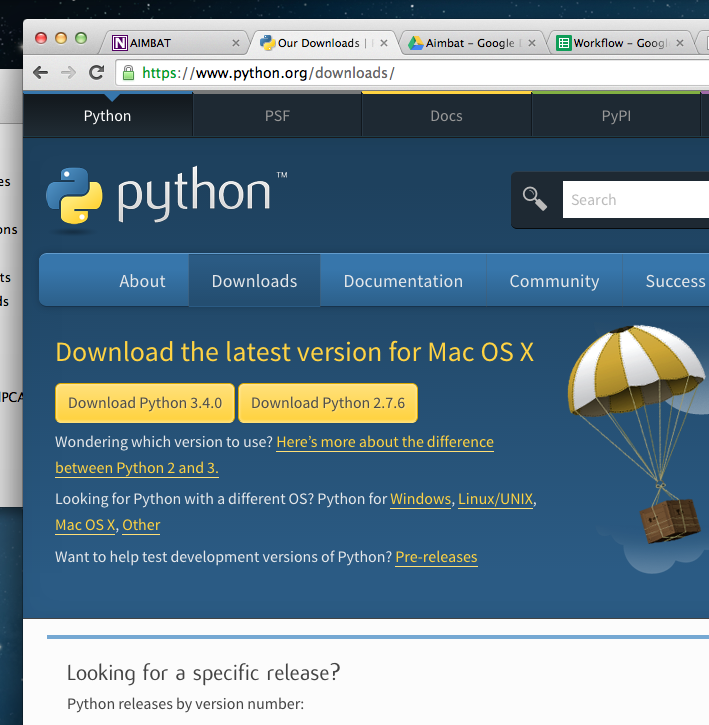
\includegraphics[width=0.5\textwidth]{images/python_version}
  \caption{Console}
  \label{fig:python_version}
\end{figure}

% ------------------------------------------------------------- %

\subsubsection{Macports}

Its best to use Macports \url{http://guide.macports.org/} to install the necessary python libraries for AIMBAT. 

If you just upgraded your operating system, you need to upgrade Macports and re-install the libraries as well. Follow the instructions here: \url{https://trac.macports.org/wiki/Migration}.

% ------------------------------------------------------------- %

\subsection{Installing the necessary components}

Inside the terminal, once python is install, type these commands in using sudo mode. Note you will need to enter your admin password.

\begin{verbatim}
  sudo port install python27
  sudo port install py27-numpy
  sudo port install py27-scipy
  sudo port install py27-matplotlib
  sudo port install py27-ipython
  sudo port install python_select
\end{verbatim}

Installing the last two packages is optional. \verb"ipython" is an enhanced interactive python shell.

\verb"python_select" is used to select default Python version by the following command:

\begin{verbatim}
  port select --set python python27
\end{verbatim}

You need this version, not other versions on your computer, since this is the one that has the libraries AIMBAT needs.

% ------------------------------------------------------------- %

\section{Regarding package managers}

The package manager brew caused many problems when tried. If you figured it out properly, email the authors about exactly how you did it, and we will gratefully add it to the manual. In general, the authors do not recommend trying to install the packages separately when there are Python versions that will come with all the packages pre-installed already. 

Scipy is especially tricky as it relies on Fortran and C as well. The authors of scipy recommend these convenient ways to install it: \url{http://www.scipy.org/install.html}, by using Enthought Canopy, or Anacoda. 


% ************************************************************* %
%                                                               %
%                       INSTALLING PYTHON                       %
%                                                               %
% ************************************************************* %

% ************************************************************* %
%                                                               %
%                       INSTALLING AIMBAT                       %
%                                                               %
% ************************************************************* %


\section{Installing AIMBAT}

% ------------------------------------------------------------- %

\subsection{Getting the packages}

AIMBAT is released as a sub-package of pysmo in the name of \verb"pysmo.aimbat" along with
another sub-package pysmo.sac. The latest releases of pysmo.sac and pysmo.aimbat are
available for download at \url{http://www.earth.northwestern.edu/~xlou/aimbat.html} and Github. 

The packages should be installed into the Python site-packages directory. To find out where that is, in the python console, do

\begin{verbatim}
  import site;
  site.getsitepackages()
\end{verbatim}

Whatever is output there, lets call it \verb"<pkg-install-dir>". You can choose to install AIMBAT either locally or globally, depending on whether you want all users of the computer to have access to it.

\begin{figure}[h!]
  \centering
  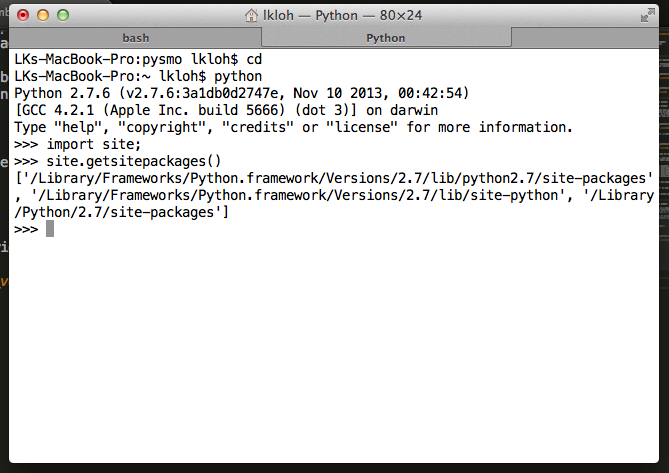
\includegraphics[width=0.5\textwidth]{images/site_package_location}
  \caption{Console}
  \label{fig:site_package_location}
\end{figure}

Make a directory called \verb"pysmo", and place the sac and aimbat directories there. 

Now that we know the location of the site-packages direction, cd into it. Call the path to it \verb"<pkg-install-dir>" Notice that in this case, the site-packages has been installed for all users on the computer, not just the current user's home directory. 

Put the two Python packages inside the directory.

% -------------------------------------------------------------------------- %

\subsection{Installing pysmo.sac}

Python module \verb"Distutils" is used to write a setup.py script to build, distribute, and install \verb"pysmo.sac". In the directory \verb"<pkg-install-dir>/pysmo-sac-0.5>", type 

\begin{verbatim}
  sudo python setup.py build
  sudo python setup.py install
\end{verbatim}

to install it and its package information file \verb"<pysmo.sac-0.5-py2.7.egg-info" to the global site-packages directory \verb"<prefix>/lib/python2.7/site-packages", which is the same as Numpy, Scipy, and Matplotlib.

If you don't have write permission to the global site-packages directory, use the \verb"'--user'" option to install to \verb"<userbase>/lib/python2.7/site-packages":

\begin{verbatim}
  python setup.py install --user
\end{verbatim}

This will install it to your home directory only, not for all users on the computer. 

If you successfully installed the \verb"sac" module, in the python console, this should happen after you type \verb"from pysmo import sac": 

\begin{figure}[h!]
  \centering
  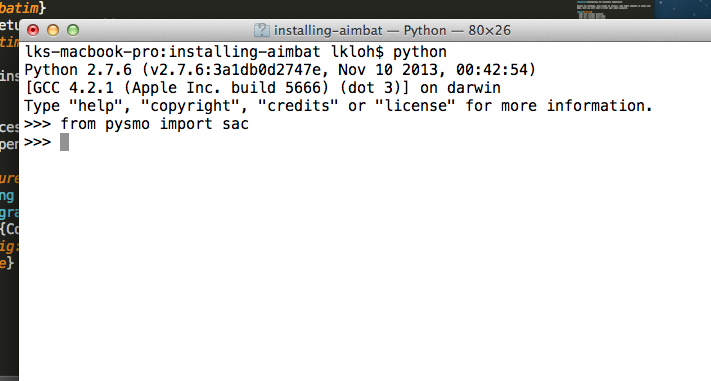
\includegraphics[width=0.5\textwidth]{images/sac_installed}
  \caption{Console}
  \label{fig:sac_installed}
\end{figure}

% ------------------------------------------------------------------------- %

\subsection{Installing pysmo.aimbat}

Three sub-directories are included in the \verb"<pkg-install-dir>/pysmo/pysmo-aimbat-0.1.2>" directory: \verb"example", \verb"scripts", and \verb"src", which contain example SAC files, Python scripts to run at the command line, and Python modules to install, respectively.

The core cross-correlation functions in \verb"pysmo.aimbat" are written in both Python/Numpy (\verb"xcorr.py") and Fortran (\verb"xcorr.f90"). Therefore, we need to use Numpy's \verb"Distutils" module for enhanced support of Fortran extension. The usage is similar to the standard Disutils. 

Note that some sort of Fortran compiler must already be installed first. Specify them in place of \verb"gfortran" in the following commands.

In the directory \verb"<pkg-install-dir>/pysmo/pysmo-aimbat-0.1.1", type

\begin{verbatim}
  sudo python setup.py build --fcompiler=gfortran
  sudo python setup.py install 
\end{verbatim}

to install the \verb"src" directory. 

Add \verb"<pkg-install-dir>/pysmo/pysmo-aimbat.0.1.2/scripts" to environment variable \verb"PATH" in a shells start-up file for command line execution of the scripts.

For Bash shell users: do \verb"export PATH=$PATH:<pkg-install-dir>/pysmo/pysmo-aimbat-0.1.2/scripts" in \verb".bashrc" files.

For C shell users, do \verb"setenv PATH=$PATH:<pkg-install-dir>/pysmo/pysmo-aimbat-0.1.2/scripts" in \verb".bashrc" files.

If AIMBAT has beenn installed, type \verb"from pysmo import aimbat" in a Python shell, and no errors should appear. 

% ************************************************************* %
%                                                               %
%                         INSTALLING SAC                        %
%                                                               %
% ************************************************************* %

\section{Seismic Analysis Code (SAC)}

AIMBAT uses Seismic Analysis Code (SAC) formatting for some of the files it runs and outputs. You can download it here: \url{http://www.iris.edu/files/sac-manual/}. To get SAC, you will need to fill out a software request form available on the IRIS website.

% ************************************************************* %
%                                                               %
%                         INSTALLING SAC                        %
%                                                               %
% ************************************************************* %



















% ------------------------------------------------------------------------- %

\end{document}

% --------------------------------- END --------------------------------- %
